\documentclass[aspectratio=169, usenames,dvipsnames, 14pt]{beamer}
\usepackage[utf8]{inputenc}
\usepackage[utf8]{inputenc}
\usepackage{multirow}
\usepackage{gensymb}
\usepackage[absolute,overlay]{textpos}
\usepackage[export]{adjustbox}
\usepackage[absolute,overlay]{textpos}  % Absolute placement of text in frame

% \usepackage[dvipsnames]{xcolor} % Testing for color of slide 11
\usepackage{listings}           % For source code fonts
\usepackage{tikz}               % For absolute image placement and shapes
\usepackage{Formatting/python_formatting}   % User defined formatting file for source codes

\usepackage{Formatting/grid_overlay}        % Grid overlay for accurate placement of images

\usetikzlibrary{calc}           % For absolute image placement
\usetikzlibrary{decorations.pathreplacing}      % For curly braces

\usetikzlibrary{arrows, positioning, shapes.geometric}

\mode<presentation>
\usetheme{Rochester}


\title{\textbf{Getting Started With OpenMDAO}}
\author{Author Number One}

\begin{document}

%---------------------------------------------------------------------
\begin{frame}
    
    \maketitle

    \tikz[remember picture, overlay] \node[anchor=center] at ($(current page.center)-(5,1)$) {\includegraphics[scale=0.15]{images/frong2.png}};

    \tikz[remember picture, overlay] \node[anchor=center] at ($(current page.center)-(-5,1)$) {\includegraphics[scale=0.17]{images/front1.png}};

    \tikz[remember picture, overlay] \node[anchor=center] at ($(current page.center)-(0,-3.7)$) {\includegraphics[scale=0.24]{images/omdao.png}};

    \tikz[remember picture, overlay] \node[anchor=center] at ($(current page.center)-(-5,3.4)$) {\includegraphics[scale=0.21]{images/michiganlogo.png}};

\end{frame}
%---------------------------------------------------------------------

\begin{frame}{Download these slides and tutorial scripts from GitHub}

    \centering
    \url{https://github.com/openmdao/openmdao\_training}

\end{frame}
%---------------------------------------------------------------------


\begin{frame}{Acknowledgements}
    \begin{itemize}
        \item \textbf{Ben Brelje}, PhD candidate at University of Michigan MDO Lab for creating version 0 of this 
        \vspace{0.5cm}
        \item \textbf{Justin Gray}, Engineer and team lead of OpenMDAO at NASA Glenn for refining this workshop
        \vspace{0.5cm}
        \item NASA ARMD’s TTT Project has supported OpenMDAO development since 2008
    \end{itemize}
    
\end{frame}
%---------------------------------------------------------------------

\begin{frame}{OpenMDAO is an open-source framework for efficient MDAO}
    \begin{itemize}
        \item Developed and supported a team at NASA Glenn since 2008
        \vspace{0.5cm}
        \item Apache 2.0 license is very permissive (no “copyleft”)
        \vspace{0.5cm}
        \item Fast enough for high-fidelity, expensive problems but easy enough for cheap conceptual models
        \vspace{0.5cm}
        \item Can be used as a framework, or a low level library for building stand alone codes
    \end{itemize}
    
\end{frame}
%---------------------------------------------------------------------

\begin{frame}{OpenMDAO is a reasonable choice for a wide array of MDAO problems}
    \begin{columns}
    
        \column[T]{0.5\textwidth}
            \begin{itemize}
                \item High-fidelity aeropropulsive optimization with RANS and CEA
                
                \uncover<2->{
                \item Medium-fidelity aerostructural optimization (VLM/beam)}
                
                \uncover<3->{
                \item Conceptual-fidelity sizing and tradespace exploration}
            \end{itemize}
        
        \column[t]{0.5\textwidth}
            
           \only<1>{ 
           \includegraphics[scale=0.28]{images/front1.png}\\
           }
           \only<2>{
           \includegraphics[scale=0.32]{images/span.png}
           }
            
            \only<3>{
            \includegraphics[scale=0.32]{images/rangeplot.png}
            }
    \end{columns}
\end{frame}

%---------------------------------------------------------------------

\begin{frame}{OpenMDAO is a reasonable choice for a wide array of MDAO problems}
        \includegraphics[scale=.27]{images/combined.png}
\end{frame}

%---------------------------------------------------------------------

\begin{frame}{Goals for today}
    \begin{itemize}
        \item Learn enough to run a useful OpenMDAO model
        \vspace{.5cm}
        \item Gain some intuition about the operating theory
        \vspace{.5cm}
        \item Get \textcolor{red}{\textbf{really excited}} about using analytic derivatives for optimization!

    \end{itemize}
    
\end{frame}
%---------------------------------------------------------------------

\begin{frame}{Overview}
    \begin{itemize}
        \item OpenMDAO intro and basics
          \begin{itemize}
            \item Lab 0: Explicit components and connections
          \end{itemize}
    \vspace{.5cm}
    
        \item Using solvers with implicit models
          \begin{itemize}
            \item Lab 1: Comparing gradient-free and gradient-based solvers
          \end{itemize}
    \vspace{.5cm}
    
        \item Optimization with and without analytic derivatives
          \begin{itemize}
              \item Lab 2: Optimizing the thickness distribution of a simple beam
          \end{itemize}
    \vspace{.5cm}
    
        \item Wrapping external codes
          \begin{itemize}
              \item Lab 3: Wrapping external codes as explicit and implicit components
          \end{itemize}
    \end{itemize}
    
\end{frame}
%---------------------------------------------------------------------
\begingroup
\setbeamercolor{background canvas}{bg=GreenYellow}
\begin{frame}{OpenMDAO intro and Basics}

    \begin{itemize}
        \item Intro and terminology 
        \vspace{0.5cm}
        \item Building explicit components and connecting them together
        \vspace{0.5cm}
        \item Lab 0: Implementing a simple explicit calculation \\(Breguet Range)
    \end{itemize}
    
\end{frame}
\endgroup
%---------------------------------------------------------------------

\begin{frame}{OpenMDAO has nice features}
    \begin{itemize}
        \item Units
          \begin{itemize}
              \item Conversions
              \item (In)compatibility checks
          \end{itemize}
\pause
\vspace{.5cm}
        \item Automatic checks for unconnected inputs
\pause
\vspace{.5cm}
        \item Interactive N2 diagrams
\pause
\vspace{.5cm}
        \item Models are Python objects (inheritance!)
    \end{itemize}
\end{frame}
%---------------------------------------------------------------------

\begin{frame}{OpenMDAO has best-in-class numerical methods}
    \begin{itemize}
        \item Efficient solvers for implicit systems
        \begin{itemize}
            \item Newton solver
            \item Nonlinear block Gauss-Seidel
        \end{itemize}
\pause
\vspace{0.5cm}
        \item Derivative computation (for gradient-based opt.)
        \begin{itemize}
            \item Forward and reverse analytic
            \item Finite difference or complex step
            \item Mixture of all!
            \end{itemize}
\pause
\vspace{0.5cm}
        \item MPI parallelization
    \end{itemize}
    
\end{frame}
%---------------------------------------------------------------------

\begin{frame}{OpenMDAO architecture}
\begin{columns}[T]
    \column{0.5 \textwidth}
        \begin{itemize}
            \item \small \textbf{Components} implement the actual model computation
        \vspace{0.5cm}
            \uncover<2->{\item \small Groups organize the model and enable hierarchical solver strategies}
        \vspace{0.5cm}
            \uncover<3->{\item \small Drivers iteritively execute the model (optimizers and DOEs)}
        \vspace{0.5cm}
            \uncover<4->{\item \small \textbf{Problem} is the top-level container}
        \end{itemize}
        
    \column{0.5 \textwidth}
        \uncover<1->{\includegraphics[scale=0.2]{images/arch1.png}}
\end{columns}
    
\end{frame}
%---------------------------------------------------------------------

\begin{frame}{ExplicitComponent class}
    \begin{columns}[T]
  
        \column{0.5 \textwidth}
            \begin{itemize}
                \item Used for doing explicit calculations
                \vspace{.5cm}
                \uncover<2->{\item Inputs $\rightarrow$ Outputs with no iteration / implicit states}
                \vspace{.5cm}
                \uncover<3->{\item Can be as simple as a one-line calculation, or as complex as an adjoint CFD solver}
            \end{itemize}

    \column{0.5 \textwidth}
        \begin{tikzpicture}[overlay]
            % \draw (2.9, -2) node [inner sep=0] {\uncover<1->{\includegraphics[scale=0.2]{images/arch1.png};}};
            \draw (2.9, -2) node [inner sep=0] {\includegraphics[scale=0.2]{images/arch1.png}};
            \draw [blue, ultra thick] (4.8,-2.7) circle (0.65cm);
            \draw[blue, very thick] (-2,1.3) -- (4.2, -2.5);
        \end{tikzpicture}
  \end{columns}
 
\end{frame}
%---------------------------------------------------------------------
% Need to have alternating white/grey lines in background
\begin{frame}{ExplicitComponent example}

    \lstinputlisting[language=Python]{SourceCodes/explicity_component_example.py}

    \pause
  
    \only<2>{
        \begin{tikzpicture}[overlay]
            \draw[red, very thick, <-] (6cm,6.3cm) to (8cm, 6.3cm);
        \end{tikzpicture}
  
        \begin{textblock*}{6cm}(9.3cm,2.35cm)
            \footnotesize \textcolor{red}{All your model components will \\ subclass OpenMDAO base classes}
        \end{textblock*}
  }
  
  \pause
  
    \only<3>{
        \begin{tikzpicture}[overlay]
            \draw[red, very thick, <-] (10.6cm,5.4cm) to (11.5cm, 5.8cm);
        \end{tikzpicture}
 
        \begin{textblock*}{6cm}(9.3cm,2.35cm)
            \footnotesize \textcolor{red}{Define any options / run flags which\\do not change during evaluation}
        \end{textblock*}
    }
    
  \pause
 
    \only<4>{
        \begin{tikzpicture}[overlay]
            \draw[red, very thick, <-] (10.6cm,4.4cm) to (11.5cm, 5.8cm);
        \end{tikzpicture}
 
        \begin{textblock*}{7cm}(8.5cm,2.2cm)
            \footnotesize \textcolor{red}{Define model inputs, output, and (optionally)\\partial derives using the setup() method.\\Called once before solve / optimization}
        \end{textblock*}
  }
 
  \pause
 
    \only<5>{
        \begin{textblock*}{7cm}(9cm,6.6cm)
            \footnotesize \textcolor{red}{Do the actual computation using compute(). Need to fill in values for all your declared outputs by the end of this method. Called every time the model is evaluated}
        \end{textblock*}
  }
  
  \pause
  
    \only<6>{
%----------------------------------------------------------------------------------------
%----------Begin the arrows and text on the last 'ExplicitComponent example' Frame-------
%----------------------------------------------------------------------------------------
        \begin{tikzpicture}[overlay]
            \draw[red,very thick, <-](4.2cm,4.3cm) to (5.8cm,6.5cm);
        \end{tikzpicture}
    
        \begin{textblock*}{5cm}(7cm,2.3cm)
            \footnotesize \textcolor{red}{Variable name}
        \end{textblock*}
%-------------%------------    
        \begin{tikzpicture}[overlay]
            \draw[red,very thick, <-](5cm,4.3cm) to (7cm,6cm);
        \end{tikzpicture}
    
        \begin{textblock*}{5cm}(7.6cm,2.7cm)
            \footnotesize \textcolor{red}{Default value (before model runs)}
        \end{textblock*}
%-------------%------------    
        \begin{tikzpicture}[overlay]
            \draw[red,very thick, <-](6.2cm,4.3cm) to (8cm,5.6cm);
        \end{tikzpicture}
    
        \begin{textblock*}{5cm}(9cm,3.1cm)
            \footnotesize \textcolor{red}{Units (need not match upstream)}
        \end{textblock*} 
%-------------%------------    
        \begin{tikzpicture}[overlay]
            \draw[red,very thick, <-](8.8cm,4.4cm) to (10.9cm,4.8cm);
        \end{tikzpicture}
    
        \begin{textblock*}{3cm}(12.3cm,3.7cm)
            \footnotesize \textcolor{red}{Human-readable description (optional)}
        \end{textblock*}    
%-------------%------------    
        \begin{tikzpicture}[overlay]
            \draw[red,very thick, <-](8.2cm,2.8cm) to (11.4cm,3.1cm);
        \end{tikzpicture}
    
        \begin{textblock*}{3cm}(12.8cm,5.7cm)
            \footnotesize \textcolor{red}{Variable dimension (in this case, a n x 1 vector)}
        \end{textblock*}    
        %-------------%------------    
        \begin{tikzpicture}[overlay]
            \draw[red,very thick, <-](6.2cm,2cm) to (8cm,2cm);
        \end{tikzpicture}
    
        \begin{textblock*}{3.6cm}(9.5cm,7.2cm)
            \footnotesize \textcolor{red}{Will default to expecting user provided analytic derivatives, but we can specify `fd` later…}
        \end{textblock*}   
  }
\end{frame}     % Error is from the source code being outside the defined area (can ignore)
%---------------------------------------------------------------------

\begin{frame}{Connecting multiple components}
\begin{columns}
    \column[T]{0.5\textwidth}
        \begin{itemize}
            \item Combine components into a Group to build models
            \vspace{0.5cm}
            \item Groups can hold other Groups, forming a hierarchy
        \end{itemize}
    
    \column[T]{0.5\textwidth}
        \includegraphics[scale=0.2]{images/arch1.png}
        \begin{tikzpicture}[overlay]
            \draw [blue, ultra thick] (-4.75,2) circle (0.55cm);
      \end{tikzpicture}
    \end{columns}
    
\end{frame}
%---------------------------------------------------------------------

\begin{frame}{Connecting multiple components}
    \lstinputlisting[language=Python]{SourceCodes/connecting_multiple_components.py}

    \only<1>{
        \begin{textblock*}{6cm}(8cm,2.7cm)
            \footnotesize \textcolor{red}{Define a model by subclassing Group}
        \end{textblock*} 
        
        \begin{tikzpicture}[overlay]
            \draw[red,very thick,<-](3.9,6.35) to (6.7,6.25);
        \end{tikzpicture}

        \begin{textblock*}{5cm}(8.3cm,7cm)
            \footnotesize \textcolor{red}{This is the model structure that is being connected}
        \end{textblock*} 
    
        \begin{tikzpicture}[overlay]        % Curly brace
            \draw [red, very thick,decorate,decoration={brace,amplitude=10pt,mirror,raise=4pt},yshift=0pt]
            (6.2,2.3) -- (6.2,3.9) node [midway,xshift=3cm] {\footnotesize $\includegraphics[scale=0.2]{images/explicit_box.png}$};
        \end{tikzpicture}
    }
    
    \pause

    \only<2>{

%-------------------------------%
        \begin{tikzpicture}[overlay]
            \draw[red, very thick, <-](4.6,5.8) to (8.5,5.2);         % Top Arrow
            \draw[red, very thick] (4.6,4) rectangle ++(3.5,0.6);  % Box at line 11, 12
            \draw[red, very thick,<-](7.9,4) to (10, 3.5);          % Bottom arrow
        \end{tikzpicture}

        \begin{textblock*}{5cm}(9.5cm,3.7cm)
            \footnotesize \textcolor{red}{Include components using the add\_subsystem (name, component) method}
        \end{textblock*}
    
        \begin{textblock*}{4cm}(11cm,5.6cm)
            \footnotesize \textcolor{red}{Python note: These are instances of a component class}
        \end{textblock*}
    }
    
    \pause %----------------------------------------
    
    \only<3>{
        \begin{tikzpicture}[overlay]
            \draw[red, very thick, <-](6.8,4.4) to (9,4.4);     %Top arrow
            \draw[red, very thick, <-](6.8,4) to (10,2.5);        % Bottom arrow
        \end{tikzpicture}
    
        \begin{textblock*}{5cm}(10cm,3.8cm)
            \footnotesize \textcolor{red}{Your custom components can be defined in the same .py file, or imported from a package for modularity}
        \end{textblock*}
    
        \begin{textblock*}{5cm}(11cm,7cm)
            \footnotesize \textcolor{red}{Specify flags/options now}
        \end{textblock*}
    }
    
    \pause %----------------------------------------
    
    \only<4>{
        \tikz[overlay]
            \draw [red, very thick,decorate,decoration={brace,amplitude=10pt,mirror,raise=4pt},yshift=0pt]
            (6.2,2.3) -- (6.2,3.9) node [midway,xshift=4.45cm] {};
        
        \begin{textblock*}{5cm}(8cm,6.1cm)
            \footnotesize \textcolor{red}{Connect parameters using the connect(from, to) method}
        \end{textblock*}

        \tikz[overlay]        % Connection boxes image
            \node[anchor=center] at ($(current page.center)-(-3,-0.5)$)
            {\includegraphics[scale=0.22]{images/explicit_box.png}};
    }
    
    \pause %----------------------------------------
    
    \only<5>{
        \begin{textblock*}{5cm}(10cm,6cm)
            \footnotesize \textcolor{red}{Note the namespace / address string\: component\_name.variable}
        \end{textblock*}   
        
        \tikz[overlay]
            \draw[red, very thick, <-](6.5,2.6) to (8.5,2.6); 
        \tikz[overlay]
            \draw[red, very thick, <-](2.65,0.5) to (8.45,2.5);
    }
    
    \pause %----------------------------------------
    
    \only<6>{
        \begin{tikzpicture}[overlay]            
            % Problem image
            \node[anchor=center] at ($(current page.center)-(-4.5,-0.5)$)
            {\includegraphics[scale=0.15]{images/arch1.png}};
            
            % Circle on image
            \draw [red, ultra thick] (12.55,5.3) circle (0.45cm);
            
            % Rectangle
            \draw [red, ultra thick](0.4,2.1) rectangle (5,1.5);              % Format: (x1,y1) rectangle (x2,y2)
            
            % Dotted line connecting circle and rectangle
            \draw[dotted, red, ultra thick] (5,2.1) -- (12,5.3);
        \end{tikzpicture}
        
        \begin{textblock*}{6cm}(7cm,7.5cm)
            \footnotesize \textcolor{red}{When you run an MDA/MDO problem, you will add one top-level Group instance to the problem}
        \end{textblock*}
    }
    
\end{frame}

%---------------------------------------------------------------------%
%---------------------------------------------------------------------%

\begin{frame}{Another way to connect…}
    \begin{itemize}
        \item If parameters are widely used among many components, writing many connect() statements can be tedious
        \item Variable \textit{promotion} is another way to make connections
    \end{itemize}
    \vspace{0.75cm}
    
    % import python source code from file
    \lstinputlisting[firstline=1, lastline=12, language=Python]{SourceCodes/another_way_to_connect.py}
    
    % Rectangle at line 11
    \tikz[overlay]
        \draw[red, very thick] (6.7,0.8) rectangle (13.5,1.2);
        
\end{frame}

%---------------------------------------------------------------------%
%---------------------------------------------------------------------%

\begin{frame}{What does variable promotion do?}
    \begin{itemize}
        \item Creates an alias for the variable one level up in the namespace 
            \begin{itemize}
                \item (atmos.h - h)
                \item (lift.rho - rho)
            \end{itemize}
        \item Automatically connects any matching I/O variable names
        \item Promote variables with wildcard (e.g. *\_\textcolor{blue}{in} or just *)
    \end{itemize}
    
    \lstinputlisting[firstline=1, lastline=12, language=Python]{SourceCodes/another_way_to_connect.py}
    
    % Rectangle at line 11
    \tikz[overlay]
        \draw[red, very thick] (6.7,0.8) rectangle (13.5,1.2);
    
\end{frame}

%---------------------------------------------------------------------%
%---------------------------------------------------------------------%

\begin{frame}{What does variable promotion do?}
    \lstinputlisting[language=Python]{SourceCodes/another_way_to_connect.py}
    
    \begin{tikzpicture}[overlay]
        \draw[red, very thick] (8.4,4.9) rectangle (13,5.25);      % Top Box
        \draw[red, very thick] (8.2,3.05) rectangle (12.9,3.45);    % Middle box
        \draw [red, ultra thick](0.4,1.1) rectangle (4,1.7);        % Bottom box
        \node[anchor=center] at ($(current page.center)-(-3,3)$)    % Image
            {\includegraphics[scale=0.25]{images/explicit_box.png}};
    \end{tikzpicture}
    
        \begin{textblock*}{4cm}(10cm,4cm)
            \footnotesize \textcolor{red}{Input/output connection established automatically}
        \end{textblock*}
\end{frame}

%---------------------------------------------------------------------%
%---------------------------------------------------------------------%

\begin{frame}{What does variable promotion do?}
    \lstinputlisting[language=Python]{SourceCodes/another_way_to_connect_2.py}
    
    \only<1>{
        \begin{textblock*}{5cm}(9cm,2.8cm)
            \footnotesize \textcolor{red}{Multiple promoted outputs with same name: not allowed (will raise an exception)}
        \end{textblock*}
        
        \begin{tikzpicture}[overlay]
            \draw[red, very thick] (8.2,3.05-0.5) rectangle (12.9,2.95);    % Top box
            \draw[red, very thick] (8.35,2.05-0.5) rectangle (11.65,1.98);    % Bottom box
        \end{tikzpicture}
        

    }
    
    \pause
    
    \only<2>{
        \begin{tikzpicture}[overlay]
            \draw[red, very thick] (8.25,0.5) rectangle (13.1,1.2);    % Top box
        \end{tikzpicture}
        
        \begin{textblock*}{6cm}(8cm,7.5cm)
            \footnotesize \textcolor{red}{Multiple promoted inputs with identical name: OK and encouraged (all connections automatically made)}
        \end{textblock*}
    
    }
    
\end{frame}

%---------------------------------------------------------------------%
%---------------------------------------------------------------------%

\begin{frame}{What does variable promotion do?}
    \lstinputlisting[language=Python]{SourceCodes/connecting_multiple_components_2.py}
    
    \tikz[overlay]
        \draw[red,very thick, <-] (5.5,.6) to (8,0.15);      % Left Arrow
    \tikz[overlay]
        \draw[red, very thick, <-] (10.8,0.9) to (9,0.15);   % Right Arrow
       
    \begin{textblock*}{5cm}(8.3cm, 7.4cm)
        \footnotesize \textcolor{red}{Mixing promotion with connect statements:allowed / appropriate}
    \end{textblock*}
\end{frame}

%---------------------------------------------------------------------%
%---------------------------------------------------------------------%

\begin{frame}{Lab 0: Implementing simple explicit calculations (Breguet Range)}
    \begin{itemize}
        \item Install OpenMDAO 
        \vspace{0.5cm}
        \item Write your first component 
        \vspace{0.5cm}
        \item World domination!
    \end{itemize}
    
\end{frame}

%---------------------------------------------------------------------%
%---------------------------------------------------------------------%

\begin{frame}{Lab 0.a: Install}
    \begin{itemize}
        \item Open cmd prompt
        \vspace{0.25cm}
        \item Internet install: \texttt{pip install openmdao}
        \vspace{0.25cm}
        \item Local Install:
            \begin{itemize}
                \item cd to wherever OpenMDAO is downloaded: \texttt{'pip install .'} \textcolor{red}{(note the period)}
                \item This installs from local source files, not PyPI
            \end{itemize}
        \vspace{0.25cm}
        \item cd ../openmdao\_training
        \vspace{0.25cm}
        \item \texttt{\textcolor{red}{python} paraboloid.py}
            \begin{itemize}
                \item If this works without error, your installation should be good
            \end{itemize}
    \end{itemize}
\end{frame}

%---------------------------------------------------------------------%
%---------------------------------------------------------------------%

\begin{frame}{Lab 0.b: Aircraft Range}
    \begin{itemize}
        \item Open \texttt{lab\_0\_template.py} in a text editor or IDE and rename it to \texttt{lab\_0.py}
        % \vspace{0.25cm}
        
        \item The \texttt{BreguetRange} component implements the electric Breguet equation: 
        
        \begin{equation}
          \small R_b= \frac{L}{D}\eta_e \eta_int \eta_p \frac{e_b}{g} \frac{m_b}{m_TO} 
        \end{equation}
        % \vspace{0.1cm}
        
        \begin{equation}
          \small m_TO = m_{empty} + m_{payload} + m_{battery}
        \end{equation}
        % \vspace{0.1cm}
        
        \item Your goal is to compute the maximum range of an airplane given a certain payload
    \end{itemize}
\end{frame}

%---------------------------------------------------------------------%
%---------------------------------------------------------------------%

\begin{frame}{Lab 0.b: Aircraft Range}
    \begin{itemize}
        \item Complete the TODOs in the \texttt{BatteryWeight} component
        \vspace{0.3cm}
        \item Complete the TODOs in the \texttt{ElecRangeGroup} definition by connecting the two components
        \vspace{0.3cm}
        \item \texttt{cd} into project folder to check and run the model
            \begin{itemize}
                \item \texttt{openmdao view\_model lab\_0.py}  (creates model diagram)
                \item \texttt{python lab\_0.py}               (runs the model)
            \end{itemize}
            \vspace{0.3cm}
        \item Answer key in the \texttt{lab\_0\_solution.py} file (don’t cheat!)
    \end{itemize}
\end{frame}

%---------------------------------------------------------------------%
%---------------------------------------------------------------------%

\begin{frame}{Lab 0.b: Aircraft Range}
    \begin{itemize}
        \item \texttt{openmdao view\_model lab\_0.py}
        \item If you forgot any connections, you’ll see some red
    \end{itemize}
    
    \includegraphics[scale=0.21]{images/lab_0_N2.png}
    
    \begin{textblock*}{4cm}(11cm,4cm)
        \small \textcolor{red}{All the red boxes represent unconnected inputs to components.}
    \end{textblock*}
    
    \begin{textblock*}{4cm}(11cm,6cm)
        \small Use explicit connection or variable promotion to get rid of all the red
    \end{textblock*}
\end{frame}

%---------------------------------------------------------------------%
%---------------------------------------------------------------------%

\begin{frame}{Lab 0.b: The n2 is your best friend!}
    \vspace{1cm}     % Move image down
    
    % N2 Diagram and the Legend side by side
    \begin{columns}
        \column[T]{0.8\textwidth}
            \includegraphics[scale=0.3]{images/n2_48.PNG}  % N2 diagram
        \column[T]{0.2\textwidth}
            \hspace{-2cm}
            \includegraphics[scale=0.26]{images/n2_legend.png}
    \end{columns}
    
    % Begin all text on the frame
    \begin{textblock*}{4.25cm}(3cm,2.3cm)
        \footnotesize \textcolor{red}{\textbf{Model hierarchy (groups, components, variables}}
    \end{textblock*}
    
    \begin{textblock*}{4cm}(10cm,2.3cm)
      \footnotesize \textcolor{red}{\textbf{Linear and nonlinear solver hierarchy (more on this later…)}}
    \end{textblock*}
        
    \begin{textblock*}{3cm}(3cm,7.5cm)
      \footnotesize \textcolor{red}{\textbf{Inside a box is within a single component}}
    \end{textblock*}
    
    \begin{textblock*}{4cm}(4.6cm,5.3cm)
        \footnotesize \textcolor{red}{\textbf{Connections!}}        % Top grid-line = 2cm, ++
    \end{textblock*}
    
    % Begin all tikzpictures
    \begin{tikzpicture}[overlay]
        \draw[red,very thick, <-] (1,5.6) to (1.8,6.3);       %Left arrow
        \draw[red,very thick, <-] (7.5,5.6) to (8.9,6.3);     % Right arrow
    \end{tikzpicture}
    


\end{frame}

%---------------------------------------------------------------------%
%---------------------------------------------------------------------%

\begin{frame}{Lab 0.b: Aircraft Range}
    \begin{columns}
        \column[T]{0.5\textwidth}
            \includegraphics[scale=0.3]{images/n2_48.PNG}\newline   % N2 diagram
            \footnotesize \textcolor{red}{N2 diagram is upper-triangular:
            Pure explicit \newline computation (feed-forward)}

        \column[T]{0.4\textwidth}
            \begin{itemize}
                \item It should look like this!
                \vspace{0.5cm}
                \item \textbf{This diagram is interactive}
                \vspace{0.5cm}
                \item Right click on the components/groups to collapse and expand them
                \vspace{0.5cm}
                \item Click on any black colored square to trace connections between components
            \end{itemize}
    \end{columns}
\end{frame}         % Error is from the image being outside of the column fram (can ignore)

%---------------------------------------------------------------------%
%---------------------------------------------------------------------%

\begin{frame}{Lab 0 summary:}
    \begin{itemize}
        \item \textit{Everything we just did we can do faster in Excel.}
        \vspace{0.5cm}
        \item This is a tutorial so the models are extremely simple and cheap, but … 
        \vspace{0.25cm}
            \begin{itemize}
                \vspace{0.25cm}
                \item Real-world models have hierarchies of dozens or hundreds of logical components
                \vspace{0.25cm}
                \item Real-world models often lack a closed form solution and require some kind of solver or iteration strategy
            \end{itemize}
    \end{itemize}
\end{frame}

%---------------------------------------------------------------------%
%---------------------------------------------------------------------%

\begingroup
\setbeamercolor{background canvas}{bg=GreenYellow}
\begin{frame}{Using solvers with implicit models}

    \begin{itemize}
        \item Gradient-free solver: Nonlinear Block Gauss-Seidel (i.e. Fixed point iteration)  
        \vspace{0.5cm}
        \item Gradient-based solver: Newton’s Method
        \vspace{0.5cm}
        \item Lab 1: Simple aircraft sizing and experimenting with different solver algorithms
    \end{itemize}
\end{frame}
\endgroup

%---------------------------------------------------------------------%
%---------------------------------------------------------------------%

\begin{frame}{OpenMDAO Nonlinear Solvers}
    When a circular dependency is detected, OpenMDAO needs a solver to converge the problem:
    
    \begin{itemize}
        \item Choice 1: NonlinearBlockGS()
        \item Choice 2: NewtonSolver()
        \item Choice 3: BroydenSolver()
        \item Choice 4: NonlinearBlockJac()
    \end{itemize}
\end{frame}

%---------------------------------------------------------------------%
%---------------------------------------------------------------------%

\begin{frame}{Check out the docs for more info!}
    \begin{columns}
        % \vspace{1cm}
        \column[T]{0.5\textwidth}
            Look at the docs for OpenMDAO's standard library:
            \newline 
            
            Lots of details on all the different solvers!
            \newline 
            
            \uncover<2->{Also see sections for surrogates and helpful general purpose components!}
            
        \column[T]{0.5\textwidth}
            \includegraphics[scale=0.25]{images/documentation_53.png}
        \end{columns}
        
        \begin{tikzpicture}[overlay]
            % Arrow on the first frame
            \only<1>{\draw[red, very thick, ->](1.5,3.7) to (8.6,0.5);}  
            % Arrows on the second frame
            \uncover<2->{\draw[red, very thick, ->](4,1.4) to (8.6,1.1);
                         \draw[red, very thick, ->](4,1.4) to (8.6, 0.25);}
        \end{tikzpicture}
\end{frame}

%---------------------------------------------------------------------%
%---------------------------------------------------------------------%

\begin{frame}{Nonlinear Block Gauss-Seidel}
    % Setting up tikzpicture for all nodes, the /.style is the formatting for the respective nodes (shapes)
    \begin{tikzpicture}[overlay,
        node distance = 0cm and 0.5cm,
        model/.style = {rectangle, draw, fill=blue!60, minimum width=2cm, minimum height=2cm, align=center},
        input/.style = {rectangle, draw, fill=blue!20, minimum width=0.75cm, minimum height=0.6cm, align=center}]
        
        % Large Model Block Nodes (mod#)
        \node (mod1)  [model, xshift=5cm,     yshift=1.7cm ]   {Model 1};
        \node (mod2)  [model, below=of mod1,  xshift=2cm   ]   {Model 2};
        \node (mod3)  [model, below=of mod2,  xshift=2cm   ]   {Model 3};
        
        % Smaller input nodes on the left side (in#)
        \node (in1)   [input, left=of mod1,   yshift= 0.7cm     ]   {};
        \node (in2)   [input, below=of in1,   yshift= -0.066cm  ]   {};
        \node (in3)   [input, below=of in2,   yshift= -0.066cm  ]   {};
        
        \uncover<2->{
            \node (mod1)  [model, xshift=5cm,    yshift= 1.7cm, fill=green!40]   {Model 1};
            \node (in4)   [input, above=of mod1, yshift= 0.1cm, fill=green!40]   {};
        }
        
        \uncover<3->{
            \node (mod2)  [model, below=of mod1,   xshift= 2cm,       fill=yellow!40 ]  {Model 2};
            \node (in5)   [input, above=of mod2,   yshift= 0.1cm,     fill=yellow!40 ]  {};
            \node (in6)   [input, below=of in3,    yshift= -0.066cm,  fill=green!40  ]  {};
            \node (in7)   [input, below=of in6,    yshift= -0.066cm                  ]  {};
            \node (in8)   [input, below=of in7,    yshift= -0.066cm                  ]  {};
        }
        
        \uncover<4->{
            \node (mod3)   [model, below=of mod2,  xshift= 2cm,       fill=orange!50 ]   {Model 3};
            \node (in9)    [input, above=of mod3,  yshift= 0.1cm,     fill=orange!50   ]   {};
            \node (in10)   [input, below=of in8,   yshift= -0.066cm,  fill=green!40  ]   {};
            \node (in11)   [input, below=of in10,  yshift= -0.066cm,  fill=yellow!40 ]   {};
            \node (in12)   [input, below=of in11,  yshift= -0.066cm                  ]   {};
        }
        
        \uncover<5->{
            \node (mod1)  [model, xshift=5cm,     yshift=1.7cm,       fill=red!10     ]   {Model 1};
            \node (in1)   [input, left=of mod1,   yshift= 0.7cm,      fill=green!70   ]   {};
            \node (in2)   [input, below=of in1,   yshift= -0.066cm,   fill=yellow!70  ]   {};
            \node (in3)   [input, below=of in2,   yshift= -0.066cm,   fill=orange!70  ]   {};
            \node (in4)   [input, above=of mod1,  yshift= 0.1cm,      fill=red!10     ]   {};
        }
        
        \uncover<6->{
            \node (mod2)  [model, below=of mod1,   xshift= 2cm,       fill=green!70  ]  {Model 2};
            \node (in5)   [input, above=of mod2,   yshift= 0.1cm,     fill=green!70  ]  {};
            \node (in6)   [input, below=of in3,    yshift= -0.066cm,  fill=red!10    ]  {};
            \node (in7)   [input, below=of in6,    yshift= -0.066cm,  fill=yellow!70 ]  {};
            \node (in8)   [input, below=of in7,    yshift= -0.066cm,  fill=orange!70 ]  {};
        
        }

        % line and arrow connecting Model 3 to the input, Only on frame 1
        \only<1>{
            \draw [blue, very thick] (mod3) -- (2,-2.3);
            \draw [blue, very thick] (2,-2.3) -- (2,1.05);
            \draw [blue, very thick, ->] (2,1.05) -- (in3);
        }
    \end{tikzpicture}

% Text Blocks -------------------------------------------
    \begin{textblock*}{2cm}(13cm,3cm)
        \textbf{\textcolor{red}{Outputs}}
    \end{textblock*}
    
    \begin{textblock*}{3cm}(1cm,5cm)
        \footnotesize \textcolor{red}{\textbf{Inputs}}
    \end{textblock*}
    
    \only<1>{
        % Text describing the connection arrow
        \begin{textblock*}{3cm}(5cm,7cm)
            \textcolor{red}{Cycle connection}
        \end{textblock*}
    }
    
    \only<1,2>{
        % Text on left side
        \begin{textblock*}{3cm}(1cm,5.5cm)
            \footnotesize \textcolor{red}{Initial guess}
        \end{textblock*}
    }
    
    \only<2>{
        % Text next to Model 1 block
        \begin{textblock*}{5cm}(7.5cm,3cm)
            \small \textcolor{red}{Evaluate Model 1 using initial guess inputs }
        \end{textblock*}
    }
    
    \only<3>{
        % Text next to Model 2 block
        \begin{textblock*}{5cm}(9.5cm,5cm)
            \small \textcolor{red}{Substitute Model 1 output into state vector and run Model 2
}
        \end{textblock*}
    }
    
    \only<4>{
        % Text next to Model 3 block
        \begin{textblock*}{4.3cm}(11.3cm,7cm)
            \small \textcolor{red}{Substitute Model 2 output into state vector and run Model 3}
        \end{textblock*}
    }
    
    \only<5>{
        % Text next to Model 1 block
        \begin{textblock*}{5cm}(7.5cm,2.5cm)
            \footnotesize \textcolor{red}{Run Model 1 with input from all prior tools. Repeat until converged}
        \end{textblock*}
    }
    
        \only<6>{
        % Text next to Model 1 block
        \begin{textblock*}{5cm}(7.5cm,2.5cm)
            \footnotesize \textcolor{red}{Run Model 2 with input from all prior tools. Repeat until converged}
        \end{textblock*}
    }

\end{frame}

%---------------------------------------------------------------------%
%---------------------------------------------------------------------%

\begin{frame}{\small Newton’s Method is simple in one dimension (Gradient Based!)}
    \begin{columns}
        \column[T]{0.5\textwidth}
            \begin{equation}
                x_{n+1} = x_{n} - \frac{f(x_{n})}{f'(x_{n})}                    % Equation
            \end{equation}

        \column[T]{0.5\textwidth}
        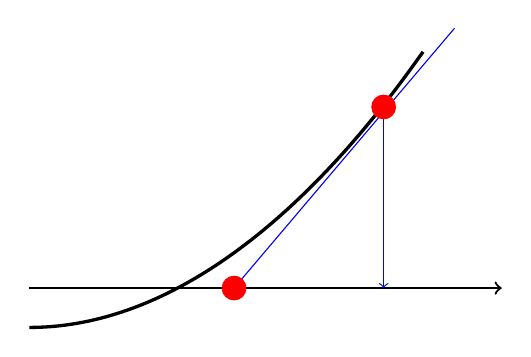
\begin{tikzpicture}
            \draw       [black, very thick]     (0,-0.5) parabola (5,3);        % parabola
            \draw       [black, thick, ->]      (0,0) to (6,0);                 % X-axis
            \draw       [blue, thin]            (2.6, 0) -- (5.4, 3.3);         % Intersection line
            \draw       [blue, ->]              (4.5, 2.3) to (4.5, 0);         % Xn arrow
            \filldraw   [red]                   (4.5,2.3) circle (0.15cm);      % Top red circle
            \filldraw   [red]                   (2.6,0) circle (0.15cm);        % Lower red circle
        \end{tikzpicture}
        
    \end{columns}
    
    % Begin text blocks
    \begin{textblock*}{3cm}(10cm, 3.5cm)
        \small \textcolor{red}{Slope = $f'(x_{n})$}
    \end{textblock*}
    
    \begin{textblock*}{3cm}(13cm, 5.5cm)
        \small \textcolor{red}{$f(x_{n})$}
    \end{textblock*}
    
    \begin{textblock*}{3cm}(12.8cm, 7.15cm)
        \small \textcolor{red}{$x_{n}$}
    \end{textblock*}
    
    \begin{textblock*}{3cm}(11cm, 7.15cm)
        \small \textcolor{red}{$x_{n+1}$}
    \end{textblock*}
\end{frame}

%---------------------------------------------------------------------%
%---------------------------------------------------------------------%

\begin{frame}{Newton Solver for multiple dimensions is a bit more complex}
    % Matrix representations on left side of frame
    \begin{columns}
    \column[]{0.25\textwidth}
        \vspace{-7cm}
        
\begin{tikzpicture}[overlay,    
            node distance = 0cm and 0.1cm,
            big/.style = {rectangle, draw, fill=blue!60, minimum width=1.5cm, minimum height=1.5cm, align=center},
            small/.style = {rectangle, draw, fill=blue!60, minimum width=0.5cm, minimum height=1.5cm,    align=center},
            txt/.style={}]
        
            Note: location of the node matters!
            \node (big1)    [big, xshift=.6cm,   yshift= 0cm]   {};
            \node (small1)  [small, right=of big1           ]   {};
            \node (textA)   [txt,  above=of big1           ]   {\textcolor{red}{$n_{y}$}};
            \node (textB)   [txt,  left= of big1           ]   {\textcolor{red}{$n_{y}$}};
            \node (text_eq) [txt,  right=of small1         ]   {\textbf{\textcolor{red}{=}}};
            \node (small2)  [small, right=of text_eq        ]   {};
            \node (textC)   [txt,  above=of small1         ]   {\textcolor{red}{1}};
            \node (textD)   [txt,  above=of small2         ]   {\textcolor{red}{1}};
            \node (textE)   [txt, right=of small2          ]   {\textcolor{red}{$n_{y}$}};
        \end{tikzpicture}
    
    \column[T]{0.33\textwidth}
    \hspace{-1cm}
    \begin{small}
        \begin{equation*}
            R(x,y)=0
        \end{equation*} 
        \begin{equation*}
          \hspace{-1cm} R(x,y + \delta y) = R(x,y) + \frac{\partial R}{\partial y} \delta y + HOT 
        \end{equation*} 
        \begin{equation*}
            0 = R(x,y) + \frac{\partial R}{\partial y} \delta y
        \end{equation*} 
        \begin{equation*}
            \delta y = -\frac{\partial R^{-1}}{\partial y}R(x,y)
        \end{equation*} 
        \begin{equation*}
            \frac{\partial R}{\partial y} \delta y = -R(x,y)
        \end{equation*} 
        \begin{equation*}
          y_{n+1} = y_{n} + \delta y
        \end{equation*} 
    \end{small}
   
    
    \column[T]{0.33\textwidth}
        % Red circle around equation
        \tikz[overlay]
            \draw [red, very thick] (-3.2cm, -5cm) ellipse (2cm and 0.7cm);     
            
    % Begin the text descriptions of each equation
        \only<1>{
            \begin{textblock*}{5.5cm}(10cm, 6cm)
                \small \textcolor{red}{Drive residuals to 0 x: design variables y: implicit state variables}
            \end{textblock*}
            \tikz[overlay]
                \draw [red, very thick, ->] (1.9,-0.25) to (-2cm, -0.25);
        }
        
        \only<2>{
            \begin{textblock*}{5.5cm}(10cm, 6cm)
                \small \textcolor{red}{Do a Taylor series with respect to the current point}
            \end{textblock*}
            \tikz[overlay]
                \draw [red, very thick, ->] (2.9,-1.25) to (0.25cm, -1.25);
        }
        
        \only<3>{
            \begin{textblock*}{5.5cm}(10cm, 6cm)
                \small \textcolor{red}{We want residuals to be 0 at the next iteration y + dy}
            \end{textblock*}
            \tikz[overlay]
                \draw [red, very thick, ->] (2.9,-2.5) to (-1cm, -2.5);
        }
        
        \only<4>{
            \begin{textblock*}{5.5cm}(10cm, 6cm)
                \small \textcolor{red}{Solve for dy that would drive the linearize residuals to 0}
            \end{textblock*}
            \tikz[overlay]
                \draw [red, very thick, ->] (-0.8,-3.6) to (-1.2cm, -3.6);
        }
        
        \only<5>{
            \begin{textblock*}{5.5cm}(10cm, 6cm)
                \small \textcolor{red}{But we don’t actually invert. Just solve this linear system}
            \end{textblock*}
            \tikz[overlay]
                \draw [red, very thick, ->] (1,-5) to (-1cm, -5);
        }
        
        \only<6>{
            \begin{textblock*}{5.5cm}(10cm, 6cm)
                \small \textcolor{red}{Then take a step. Repeat from top until converged}
            \end{textblock*}
            \tikz[overlay]
                \draw [red, very thick, ->] (1,-6) to (-1.5cm, -6);
        }
        
    \end{columns}
    
\end{frame}

% %---------------------------------------------------------------------%
% %---------------------------------------------------------------------%

\begin{frame}{Newton Solver needs some partial derivatives! }

    % Matrix representations on left side of frame
    \vspace{1cm}
    \begin{centering}
        \begin{tikzpicture}[overlay,    
            node distance = 0cm and 0.1cm,
            big/.style = {rectangle, draw, fill=blue!60, minimum width=1.5cm, minimum height=1.5cm, align=center},
            small/.style = {rectangle, draw, fill=blue!60, minimum width=0.5cm, minimum height=1.5cm,    align=center},
            txt/.style={}]
        
            % Note: location of the node matters!
            \node (big1)    [big, xshift=6cm ]   {};
            \node (small1)  [small, right=of big1          ]   {};
            \node (textA)   [txt,  above=of big1           ]   {\textcolor{red}{$n_{y}$}};
            \node (textB)   [txt,  left= of big1           ]   {\textcolor{red}{$n_{y}$}};
            \node (text_eq) [txt,  right=of small1         ]   {\textbf{\textcolor{red}{=}}};
            \node (small2)  [small, right=of text_eq       ]   {};
            \node (textC)   [txt,  above=of small1         ]   {\textcolor{red}{1}};
            \node (textD)   [txt,  above=of small2         ]   {\textcolor{red}{1}};
            \node (textE)   [txt, right=of small2          ]   {\textcolor{red}{$n_{y}$}};
        \end{tikzpicture}
        \end{centering}
        
    \begin{centering}
        \vspace{1cm}
        \begin{equation*} 
            \frac{\partial R}{\partial y} \delta y = -R(x,y) 
        \end{equation*}
        
        \begin{equation*}
          y_{n+1} = y_{n} + \delta y 
        \end{equation*}
    \end{centering}
    
    \begin{tikzpicture}[overlay]
        \draw[red, very thick]      (5,2.5) rectangle (5.8,4);    % Red box
        \draw[red, very thick, ->]  (5.5, 4)   to (5.7, 4.8);     % Left arrow
        \draw[red, very thick, ->]  (6.2, 3.5) to (7, 4.8);       % Middle arrow
        \draw[red, very thick, ->]  (8, 3.5)   to (8.6, 4.8);     % Right arrow
    \end{tikzpicture}
    
\end{frame}

% % %---------------------------------------------------------------------%
% % %---------------------------------------------------------------------%

\begin{frame}{Partial Derivatives in OpenMDAO}
    \lstinputlisting[language=Python]{SourceCodes/Partial_Derivatives_in_OpenMDAO.py}
    
    % Textblocks for equations
    \begin{textblock*}{5.5cm}(10cm, 4cm)
        \footnotesize{
            \begin{equation*} 
                \frac{\partial R}{\partial y}\delta y = -R(x,y)
            \end{equation*}}
            
            \begin{equation*}
                y_{n+1} = y_{n} + \delta y
            \end{equation*}
    \end{textblock*}
    
    % Setting up node styles
    \tikzstyle{eqn_box} = [rectangle, draw, red, very thick, minimum width=0.6cm, minimum height=1cm, align=center]
    \tikzstyle{text_box} = [rectangle, minimum width=3cm, minimum height=1cm, text justified, draw=black, fill= white!50]
    \tikzstyle{arrow} = [red,thick,->,>=stealth, line width=1.5pt]
    \tikzstyle{line} = [red, thick, line width=1.5pt]
    
    % Beginning nodes
    \begin{tikzpicture}[overlay, node distance = 0cm and 0.1cm]
        \node(redbox) [eqn_box, xshift=10.6cm, yshift=4.2cm] {};
        
        \node(text_1) [text_box, above of=redbox, node distance=1.5cm] {\textcolor{red}{\tiny OpenMDAO assembles the Jacobian for you, from provided component partials}};
        
        \node(text_2) [text_box, left of=redbox, node distance=4cm, yshift=-.7cm] {\textcolor{red}{\tiny This tells OpenMDAO which partials exist}};
        
        \node(text_3) [text_box, below of=text_2, node distance=3.3cm, xshift=2cm] {\textcolor{red}{\tiny This tells OpenMDAO the actual values of the partials}};
        
        % Empty nodes for lines connecting to text boxes
        \coordinate[below = 0.5cm of text_2, xshift=-1.4cm] (empty2);
        \coordinate[left = 1cm of text_3, yshift=0.5cm] (empty3);
        
        % Lines and arrows connecting nodes
        \draw [arrow]   (text_1) to (redbox);
        
        \draw [line]    (empty2) to (text_2);
        \draw [arrow]   (text_2) to (redbox);
        
        \draw [line]    (empty3) to (text_3);
        \draw [arrow]   (text_3) to (redbox);
    \end{tikzpicture}
    
\end{frame}

% % %---------------------------------------------------------------------%
% % %---------------------------------------------------------------------%

\begin{frame}{Lab 1 : Aircraft Sizing}
    \begin{columns}
        \column[T]{0.4\textwidth}
            Next, we will “size” an electric aircraft for desired range
            \vspace{0.25cm}
            
            \begin{itemize}
                \item \footnotesize Open lab\_1\_template.py in a text editor or IDE and rename lab\_1.py
                \item \footnotesize Check the model by building an N2 diagram
                \item \footnotesize This system is implicit (because it has a cycle) but has no implicit components
            \end{itemize}

        \column[T]{0.5\textwidth}
            \includegraphics[scale=0.25]{images/slide_65_image.PNG}
    \end{columns}
\end{frame}
    
% %---------------------------------------------------------------------%
% %---------------------------------------------------------------------%

\begin{frame}{Lab 1 : Aircraft Sizing}
    \begin{itemize}
        \item Run the model as-is using NLBGS (python lab\_1.py)
            \begin{itemize}
                \item The numbers that print out are the absolute and relative residuals
            \end{itemize}
            
        \vspace{0.25cm}
        \item Change the empty weight fraction to 0.55 
            \begin{itemize}
                \item check out the ExecComp
            \end{itemize}
            
        \vspace{0.25cm}
        \item Try using the Newton solver (~ Line 124). What happens?
            \begin{itemize}
                \item Check your partial derivatives (~ Line 173)
                \item Fix the partial derivatives of the incorrect components
                \item Which solver uses fewer iterations?
            \end{itemize}
            
        \vspace{0.25cm}
        \item Print all the inputs and outputs (~ Line 178, 179)
    \end{itemize}
    
\end{frame}

%---------------------------------------------------------------------%
%---------------------------------------------------------------------%

\begin{frame}{check partials output}

\includegraphics[scale=0.25]{images/slide_67_image.PNG}
    
\end{frame}

%---------------------------------------------------------------------%
%---------------------------------------------------------------------%

\begin{frame}{Lab 1 : Aircraft Sizing continued}
    \begin{columns}
    \hspace{-1cm}
        \column[T]{0.6\textwidth}
    
            \begin{itemize}
                \item Switch back to the Gauss-Seidel solver
                
                \vspace{0.25cm}
                \item Switch to the WeightBuildImplicit component

                    \begin{itemize}
                        \item Solves for TOW by forcing design range equal to analyzed range
                        \item What happens when you run the model? Why?
                        \item Try the Newton solver
                    \end{itemize}
            \end{itemize}
            
        \column[T]{0.5\textwidth}
            \includegraphics[scale=0.24]{images/slide_68_image.PNG}
    \end{columns}
\end{frame}
    
% %---------------------------------------------------------------------%
% %---------------------------------------------------------------------%

\begingroup
\setbeamercolor{background canvas}{bg=GreenYellow}
\begin{frame}{Optimization with and without analytic derivatives}

    \begin{itemize}
        \item High level introduction to different methods of computing derivatives
        \vspace{0.5cm}
        \item Lab 2: Optimization of a FEM for a cantilever beam
    \end{itemize}
    
\end{frame}
\endgroup

% %---------------------------------------------------------------------%
% %---------------------------------------------------------------------%

\begin{frame}{Optimization}
    \begin{columns}
        \column[T]{0.5\textwidth}
            \begin{itemize}
                \item OpenMDAO is capable of evaluating DOEs just like ModelCenter, but…
                \item Gradient based optimization is A LOT faster! 
                \item So we need \textbf{total derivatives} across the whole model: 
            \end{itemize}
            
        \column[T]{0.5\textwidth}
            \begin{equation*}
                \hspace{-3cm} \vspace{-0.5cm} \frac{df(x)}{dx}
            \end{equation*}
            
            \begin{tikzpicture}[overlay, node distance = 0cm and 0.1cm]
                \tikzstyle{arrow} = [red, line width=1.5pt, ->, >=stealth]
                \tikzstyle{text_box} = [rectangle, minimum width=1cm, minimum height=1cm, text justified, fill= white!50]
                
                \node(image)    [text_box, xshift=3cm, yshift=-0.5cm] {\includegraphics[scale=0.2]{images/slide_70_image.PNG}};
                
                \node(eqn1)     [text_box, right of=image, node distance=3.4cm] {f(x)};
                
                \node(eqn2)     [text_box, below of=image, node distance=3.3cm] {$\displaystyle{\frac{df(x)}{dx}}$  \hspace{1cm} \textcolor{red}{??}};
                
                \node(circ1) [below of=eqn2, circle,red, thick, draw, minimum size=2cm, xshift=-1cm] (c) {};
                
                \draw [arrow]   (image) to (eqn1);
            \end{tikzpicture}
            
    \end{columns}
    
\end{frame}

% %---------------------------------------------------------------------%
% %---------------------------------------------------------------------%

\begin{frame}{Finite difference is easy}
    \begin{columns}
        \column[T]{0.5\textwidth}
            \small{
           \begin{equation*}
                {\frac{\partial F}{\partial x_{j}} = \frac{F(x+xe_{j}h) - F(x)}{h} + \theta (h)}
           \end{equation*}
        
            \vspace{1cm}
        
            f(x+h)      \hspace{.25cm}      + 1.2345678901234\textcolor{red}{31}\\
            f(x)        \hspace{.75cm}      + 1.234567890123456\\
            $\Delta f$    \hspace{1cm}        - 0.000000000000025
            }
        
        \column[T]{0.5\textwidth}
            \begin{tikzpicture}[overlay, node distance=0m and 0 cm]
                \tikzstyle{axes} = [black, line width = 1.5pt, ->, >=stealth]
                \tikzstyle{dotted} = [dashed]
                \tikzstyle{blueline} = [blue, thick]
                \tikzstyle{redline} = [red, thick]
                \tikzstyle{text_box} = [rectangle, minimum width=1cm, minimum height=1cm, text justified]
                
                % To move the image, change the 'yshift' value, and/or 'xshift'
                \node(origin) [circle, fill, inner sep=1.5pt, yshift=-4.5cm, xshift=1cm] {};
                \coordinate[above = 5cm of origin] (y);
                \coordinate[right = 5cm of origin] (x);
   
                \draw [axes]   (origin) to (y);
                \draw [axes]   (origin) to (x);
                
                % coordinates along x and y axes
                \coordinate [above = 2.5cm of origin]   (fx);
                \coordinate [above=0.75cm of origin]    (fxh);
                \coordinate [right=2cm of origin]       (x_cord);
                \coordinate [right=3.5cm of origin]     (xh);
                \coordinate [right=3.6cm of fxh]        (fxh_xh_int);
                
                % intersection point of curved line
                \node(int) [right=2cm of fx, circle, fill, inner sep=2pt] {};
                
                % dotted lines
                \draw[dotted] (fx) to (int);
                \draw[dotted] (int) to (x_cord);
                \draw[dotted] (fxh) to (fxh_xh_int);
                \draw[dotted] (xh) to (fxh_xh_int);
                
                % red line
                \draw[redline] (fxh_xh_int) to (int);
                
                % blue line
                \coordinate [below=2cm of int, xshift=0.7cm] (blue_bot);
                \coordinate [above=2cm of int, xshift=-0.7cm] (blue_top);
                \draw[blueline] (blue_bot) to (blue_top);
                
                % Curved plot
                \coordinate [above=2cm of fx, xshift=0.5cm] (top);
                \coordinate [right=1cm of xh, yshift=0.6cm] (bottom);
                \draw [very thick] (top) to [out=-20,in=110] (int) to [out=290,in=180] (bottom);
                
                 \node(y_fx) [text_box, left of=fx, node distance=0.5cm] {\footnotesize f(x)} {};
                 \node(y_fxh) [text_box, left of=fxh, node distance=0.75cm] {\footnotesize f(x+h)} {};
                 \node(xx) [text_box, below of=x_cord, node distance=0.3cm] {\footnotesize x} {};
                 \node(xxh) [text_box, below of=xh, node distance=0.3cm] {\footnotesize x+h} {};
                 
            \end{tikzpicture}
    \end{columns}
    
\end{frame}

% \begin{frame}{Finite difference is easy, but. . .} 
% 
% \begin{columns}
%     \column[T]{0.5 \textwidth}
%         \begin{itemize}
%             \item Treats your model as a black-box
%             \item Expensive
%             \item Accuracy can be bad, especially close to the optimal point
%         \end{itemize}
% 
%         \vspace{-0.5cm}
% 
%         \begin{equation*}
%             \frac{\partial \textbf{F}}{\partial x_{j}} =\frac{ \textbf{F}(\textbf{x}+e_{j}h)-\textbf{F(x)}}{h} +\Theta (h)
%         \end{equation*}
% 
%     \column[T]{0.5 \textwidth}
%     \includegraphics[scale=0.3]{images/slide73.png}
% 
% \end{columns}
% 
% \end{frame}
    
    
\begin{frame}{Friends don’t let friends finite difference across solvers!}
\textbf{\small Seriously. Don’t do this unless you really have to.}

\begin{itemize}
    \item \small It’s expensive (make your solver tolerances really tight)
    \item \small It’s inaccurate
    \item \small It will probably make your optimization converge slowly!
\end{itemize}

\small Lots of papers on this topic: 

\tiny {
\begin{itemize}
\item \textbf{E. S. Hendricks and J. S. Gray, “Pycycle: a tool for efficient optimization of gas turbine engine cycles,”Aerospace, vol. 6, iss. 87, 2019.}

\item E. S. Hendricks, “A multi-level multi-design point approach for gas turbine cycle and turbine conceptual design,” PhD Thesis, 2017.

\item J. S. Gray, T. A. Hearn, K. T. Moore, J. Hwang, J. Martins, and A. Ning, “Automatic Evaluation of Multidisciplinary Derivatives Using a Graph-Based Problem Formulation in OpenMDAO,” in15th AIAA/ISSMO Multidisciplinary Analysis and Optimization Conference, 2014.

\item J. S. Gray, K. T. Moore, T. A. Hearn, and B. A. Naylor, “Standard Platform for Benchmarking Multidisciplinary Design Analysis and Optimization Architectures,”AIAA Journal, vol. 51, iss. 10, p. 2380–2394, 2013.

\item C. Marriage and Martins, J. R. R. A. “Reconfigurable Semi-Analytic Sensitivity Methods and MDO Architectures Within the $\pi$MDO Framework”, in Proceedings of the 12th AIAA/ISSMO Multidisciplinary Analysis and Optimization Conference, Victoria, BC, 2008
\end{itemize}
}

\end{frame}
% ------------------------------------------
% ------------------------------------------

% \begin{frame}{Complex step is more accurate than FD, but}
%     \begin{columns}
%         \column[T]{0.5 \textwidth}
%             \begin{itemize}
%                 \item Treats your models as a gray-box (might require code modification
%                 \item Even more expensive
%                 \item some functions are tricky ...
%                     \begin{itemize}
%                         \item min(), max(), abs() can cause issues
%                     \end{itemize}
%             \end{itemize}
% 
%             \vspace{-0.5cm}
% 
%             \begin{equation*}
%                 \frac{\partial \textbf{F}}{\partial x_{j}} =\frac{Im(\textbf{F}(\textbf{x}+ihe_{j}))}{h} +\Theta (h^{2})
%             \end{equation*}
% 
%         \column[T]{0.5 \textwidth}
%             \includegraphics[scale=0.27]{images/slide75.png}
%     \end{columns}
% 
% \end{frame}    


% %---------------------------------------------------------------------%
% %---------------------------------------------------------------------%

% \begin{frame}{Analytic derivatives are both fast and accurate!}
% \begin{columns}
%     \column[T]{0.5 \textwidth}
%         \includegraphics[scale=0.25]{images/slide76.png}
% 
%     \column[T]{0.5 \textwidth}
%         \vspace{2cm}
%         \begin{equation*}
%             \frac{df}{dx} = \frac{\partial f}{\partial y_{b}} \frac{\partial y_{b}}{\partial y_{a}} \frac{\partial y_{a}}{\partial x}
%         \end{equation*}
% \end{columns}
% 
% \end{frame}

% %---------------------------------------------------------------------%
% %---------------------------------------------------------------------%

% \begin{frame}{What about models with coupling?}
% \centering
% \includegraphics[scale=0.25]{images/slide77.png}
% 
% \end{frame}

% %---------------------------------------------------------------------%
% %---------------------------------------------------------------------%

% \begin{frame}{How do you differentiate through this convergence loop? }
% \begin{columns}
%     \column[T]{0.4 \textwidth}
%         \includegraphics[scale=0.2]{images/slide78.png}
% 
%     \column[T]{0.6 \textwidth}
%         \begin{itemize}
%             \item We'll need a nonlinear solver to converge this coupling
%             \vspace{0.5cm}
%             \item The solver loop changes the way you compute analytic derivatives
%         \end{itemize}
% \end{columns}
% 
% \end{frame}

% %---------------------------------------------------------------------%
% %---------------------------------------------------------------------%
% \begin{frame}{Manually computing analytic derivatives for coupled models takes a lot of work}
% \begin{columns}
%     \column[T]{0.35 \textwidth}
%         \includegraphics[scale=0.2]{images/slide79.png}
% 
%     \column[T]{0.65 \textwidth}
% 
%        \begin{equation*}
%             \frac{df}{dx} = \frac{\partial f}{\partial y_{b}} \frac{\partial y_{b}}{\partial y_{a}} \frac{\partial y_{a}}{\partial x} + \frac{\partial f}{\partial y_{b}} \frac{\partial y_{b}}{dx} + \frac{\partial y_{b}}{dx} + \frac{\partial f}{\partial y_{a}} \frac{dy_{a}}{dx}
%         \end{equation*}
% \end{columns}
% 
% \end{frame}

% %---------------------------------------------------------------------%
% %---------------------------------------------------------------------%

% \begin{frame}{How to compute these extra terms?}
% \begin{columns}
%     \column[T]{0.35 \textwidth}
%         \includegraphics[scale=0.2]{images/slide79.png}
% 
%     \column[T]{0.65 \textwidth}
% 
%        \begin{equation*}
%             \frac{df}{dx} = \frac{\partial f}{\partial y_{b}} \frac{\partial y_{b}}{\partial y_{a}} \frac{\partial y_{a}}{\partial x} + \frac{\partial f}{\partial y_{b}} \frac{\partial y_{b}}{dx} + \frac{\partial y_{b}}{dx} + \frac{\partial f}{\partial y_{a}} \frac{dy_{a}}{dx}
%         \end{equation*}
% 
% 
%     \begin{tikzpicture}[overlay, node distance=0m and 0 cm]
%         \tikzstyle{red_box} = [rectangle, draw, red, very thick, minimum width=0.7cm, minimum height=1.4cm, align=center]
%         \tikzstyle{text_box} = [rectangle, minimum width=1cm, minimum height=1cm, text justified]
% 
%         \node(text) [text_box, yshift=-2.5cm, xshift=4.5cm] {\textcolor{red}{These terms will be computed using adjoints!}};
% 
%         %  to shift red boxes, move only box 1, the lines will follow
%         \node(box1) [red_box, above of=text,  node distance=3.7cm, xshift=2.2cm] {};
%         \node(box2) [red_box, right of=box1,  node distance=2cm] {};
% 
%         \draw[red, thick] (text) -- (box1);
%         \draw[red, thick] (text) -- (box2);
% \end{tikzpicture}
% \end{columns}
% 
% \end{frame}

%---------------------------------------------------------------------%
%---------------------------------------------------------------------%


\begin{frame}{When models get really big, have fun!}
\begin{columns}
    \column[T]{0.6 \textwidth}
        \includegraphics[scale=0.5]{images/slide_81.png}
    
    \column[T]{0.4 \textwidth}
        \begin{center}
            
        
        \begin{equation*}
            \LARGE\frac{df}{dx} = ???
        \end{equation*}
        \end{center}
        Lets be honest, this is just not going to happen
    
\end{columns}
    
\end{frame}

%---------------------------------------------------------------------%
%---------------------------------------------------------------------%

\begin{frame}{OpenMDAO can compute these total derivatives for you, automatically!}
\begin{columns}
    \column[T]{0.5 \textwidth}
        \includegraphics[scale=0.5]{images/slide_81.png}
    
    \column[T]{0.5 \textwidth}
        \begin{center}

        \begin{equation*}
            \LARGE\frac{df}{dx} = [ask OpenMDAO]
        \end{equation*}
       
    \textbf{For a deep dive on the math}
            \begin{itemize}
                \item Martins and Hwang 2013
                \item Hwang and Martins 2018 
            \end{itemize}
        \end{center}
\end{columns}
    
\end{frame}

%---------------------------------------------------------------------%
%---------------------------------------------------------------------%


\begin{frame}{OpenMDAO splits total derivative computation into two steps}
\begin{columns}
    \column[T]{0.4 \textwidth}
        \includegraphics[scale=0.2]{images/slide76.png}
        
    \column[T]{0.6 \textwidth}
         1) Computing the partial derivatives for each component \newline \newline
         2) Solving a linear system for total derivatives
\end{columns}
    
\end{frame}

%---------------------------------------------------------------------%
%---------------------------------------------------------------------%

\begin{frame}{OpenMDAO splits total derivative computation into two steps}
	\begin{columns}
		\column[T]{.4 \textwidth}
			\includegraphics[scale=0.2]{images/slide76.png}
	
		\column[T]{.6 \textwidth}
			\textbf{1) Computing the partial derivatives for each component}
					\begin{itemize}
						\item Numerical approach: FD/CS
						\item Analytic approach: hand derivation or algorithmic differentiation
						\item Mix and match numerical and analytic
					\end{itemize}
			\text{You are responsible for this step,} 
			\text{but OpenMDAO can help you a bit}
	\end{columns}

	\begin{tikzpicture}[overlay]
		\draw[red, very thick, ->] (5.5, 5.5) to (0.2, 4.7);
		\draw[red, very thick, ->] (5.5, 5.5) to (1.1, 3.3);
		\draw[red, very thick, ->] (5.5, 5.5) to (2.0, 2.1);
	\end{tikzpicture}

\end{frame}

\begin{frame}{OpenMDAO splits total derivative computation into two steps}
	\begin{columns}
		\column[T]{.4 \textwidth}
			\includegraphics[scale=0.2]{images/slide76.png}
	
		\column[T]{.6 \textwidth}
			1) Computing the partial derivatives for each component \newline \newline
			\textbf{2) Solving a linear system for total derivatives}
			\newline \newline
			OpenMDAO does this automatically using a library of different linear solvers for different problems
	\end{columns}

	\begin{tikzpicture}[overlay]
		\draw[blue, ultra thick] (0.1, 4.8) to ( 0.1, 4.1);
		\draw[blue, ultra thick] (0.1, 4.1) to ( 1, 4.1);
		\draw[blue, ultra thick] (1, 4.1) to ( 1, 2.8);
		\draw[blue, ultra thick] (1, 2.8) to ( 2, 2.8);
		\draw[blue, ultra thick] (2, 2.8) to ( 2, 1.55);
		\draw[blue, ultra thick] (2, 1.55) to ( 2.8, 1.55);
	\end{tikzpicture}
\end{frame}

\begin{frame}{By using OpenMDAO's analytic derivative functionality you can}
	\begin{itemize}
		\item Efficiently solve optimization problems with thousands of design variables or thousands of constraints
		\item Get total derivatives across a complicated model by providing only partial derivatives of each component
		\item Mix and match different techniques for computing partial derivatives
	\end{itemize}
\end{frame}

\begin{frame}{Rules of thumb for computing partials}
	\begin{itemize}
		\item Fine to start out with FD partials while getting your model set up!
		\item For cheap black-box codes:		
			\begin{itemize}
				\item FD \textit{might} be ok for production runs
				\item CS is better if you can do it!
			\end{itemize}
		\item For "expensive" codes (anything with an internal solver):
			\begin{itemize}
				\item Implement as ImplicitComponent (expose the states/residuals to OpenMDAO)
				\item Can still FD the residual if you need to
				\item Analytic derivatives typically cost a lot for these components
			\end{itemize}
	\end{itemize}
\end{frame}

\begin{frame}{Optimization}
	Optimization is handled by a \texttt{Driver}
	\lstinputlisting[language=Python]{SourceCodes/optimization_example.py}


	\begin{tikzpicture}[overlay]
		\draw[red, thick, ->] (8.3, 5) to (4.8, 3.3);
		\draw[red, thick, ->] (9.1, 3.9) to (7.3, 2.5);
		\draw[red, thick, ->] (8.5, 2.3) to (7.8, 2);
		\draw[red, thick, ->] (8.5, 1.5) to (6.5, 1.6);
		\draw[red, thick, ->] (7.4, .9) to (2.3, .8);
	\end{tikzpicture}

	\begin{textblock*}{6cm}(9.5cm,4.1cm)
		\footnotesize \textcolor{red}{ScipyOptimizeDriver is what most people will use on Windows}
	\end{textblock*}
	\begin{textblock*}{6cm}(10.1cm,5.3cm)
		\footnotesize \textcolor{red}{add\_design\_var(\textit{var\_name}, lower=…, upper=…)}
	\end{textblock*}
	\begin{textblock*}{6cm}(9.5cm,6.7cm)
		\footnotesize \textcolor{red}{add\_constraint(\textit{var\_name}, lower=…, upper=…)}
	\end{textblock*}
	\begin{textblock*}{6cm}(9.5cm,7.9cm)
		\footnotesize \textcolor{red}{add\_objective(\textit{var\_name})}
	\end{textblock*}
	\begin{textblock*}{6cm}(8.5cm,8.5cm)
		\footnotesize \textcolor{red}{run\_driver instead of run\_model}
	\end{textblock*}

\end{frame}

\begin{frame}{Optimization}
	Available drivers:
	\begin{itemize}
		\item \texttt{ScipyOptimizeDriver} will work in Anaconda
			\begin{itemize}
				\item Works on Windows machines	
				\item SLSQP method is the standard constrained optimizer in OpenMDAO
			\end{itemize}
		\item \texttt{PyoptSparseDriver} is much better (SNOPT algorithm) but really only builds on Linux/MacOSX (hard to build on 					Windows, but technically possible)
	\end{itemize}
\end{frame}

\begin{frame}{Recording the optimization history}
		\begin{itemize}
			\item Often you will want to record variable values changing over the course of an optimization
			\item This is achieved using a "recorder" object
			\item This will record all the objectives, all the constraints, and all the DVs for each optimizer iteration (but no 										"intermediate variables")
			\item \underline{Can then read in the data to postprocess}
		\end{itemize}
\end{frame}

\begin{frame}{Recording the optimization history}
	\lstinputlisting[language=Python]{SourceCodes/case_recorder_example.py}
	\begin{tikzpicture}[overlay]
		\draw[red, thick, ->] (13, 3) to (4.3, .77);
		\draw[red, thick, ->] (13, 3) to (5, 3.2);
	\end{tikzpicture}
\end{frame}

\begin{frame}{Saving all the variables for the final optimized point}
	\begin{columns}
		\column[T]{.37 \textwidth}
			\begin{itemize}
				\item We don't save all the variables for every iteration to avoid huge database files
				\item This configures a secondary case type to record specific runs with all the variables
			\end{itemize}
		\column[T]{.63 \textwidth}
			\lstinputlisting[language=Python]{SourceCodes/case_recorder_example.py}
	\end{columns}

	\begin{tikzpicture}[overlay]
		\draw[red, thick, ->] (4.8, 2) to (5.5, 2.5);
		\draw[red, thick, ->] (4.8, 2) to (5.5, .5);
	\end{tikzpicture}
\end{frame}

\begin{frame}{Lab \#2: Optimization of a cantilever beam}
	\begin{columns}
		\column[T]{.4 \textwidth}
			\begin{itemize}
				\item Find the thickness distribution for a cantilever beam that minizes compliance subject to a volumn constraint
				\item Check out the other examples on your own!
			\end{itemize}
		\column[T]{.6 \textwidth}
			\includegraphics[scale=0.5]{images/beam_docs.png}
			\includegraphics[scale=0.5]{images/cantilever_beam.png}
	\end{columns}
	
	\begin{tikzpicture}[overlay]
		\draw[red, thick, ->] (5, 2) to (6.6, 2.94);
	\end{tikzpicture}
\end{frame}

\begin{frame}{Lab \#2: Simple FEM in 5 steps!}
	\begin{columns}
		\column[T]{.55 \textwidth}
			\begin{itemize}
				\item \small Break the beam into segments (0 doesn't count as a real step!)
				\item \small Compute each moment of inertia
				\item \small Compute the local stiffness matrix for each segment
				\item \small Combine all the local stiffness matrices into a global K matrix and solve the FEM
				\item \small Pull displacements from the state vector and compute compliance
				\item \small Compute beam volume
			\end{itemize}
		\column[T]{.45 \textwidth}
			\includegraphics[scale=0.38]{images/slide_105.png}
			\uncover<2->{
				\small using the \texttt{src\_indices} argument to the connect method can extract the relevant portion of the state vector
			}
	\end{columns}

	\uncover<2->{
		\begin{tikzpicture}[overlay]
			\draw[red, thick, ->] (6.75, 1.5) to (12, 3.4);
			\draw[red, thick, ->] (6.75, 1.5) to (13.15, 3.7);
			\draw[red, thick] (.5, .7) to (6.6, .7);
			\draw[red, thick] (6.6, .7) to (6.6, 1.7);
			\draw[red, thick] (6.6, 1.7) to (.5, 1.7);
			\draw[red, thick] (.5, 1.7) to (.5, .7);
		\end{tikzpicture}
	}
\end{frame}

\begin{frame}{Lab \#2: Get to it!}
	\begin{columns}
		\column[T]{.5 \textwidth}
			\begin{itemize}
				\item \small Copy the "\texttt{lab\_2\_template.py}" file to a new file called "\texttt{lab\_2.py}"
				\item \small Add components in the correct order (~line 40)
				\item \small Connect the components together (~line 48)
				\item \small Use the N2 diagram to make sure you have everything connected (no red inputs!)
			\end{itemize}
		\column[T]{.5 \textwidth}
			\begin{itemize}
				\item \small What happens if you switch to full model FD? Does it work? Try changing the FD step size...
				\item \small What about complex step?
				\item \small How does compute cost scale with \texttt{num\_elements} for different methods of computing derivatives?
				\item \small What happens if you add the components in the incorrect order?
			\end{itemize}
	\end{columns}
\end{frame}

\begingroup
\setbeamercolor{background canvas}{bg=GreenYellow}
\begin{frame}{Wrapping external codes}
	\begin{itemize}
		\item How to handle file wrappers with OpenMDAO's built in helper components
		\item Lab 3: Explicit and Implicit file wrappers
	\end{itemize}
\end{frame}
\endgroup

\begin{frame}{OpenMDAO has two file wrapper components in the standard library}
	\begin{columns}
		\column[T]{.33 \textwidth}
			\begin{itemize}
				\item \small There are lots of useful components in the standard library!
				\item \small Spines, constraint aggregation, \textbf{file wrappers}, Ax=b, Ax, etc.
				\item \small Have a look through these comps so you know what's there
			\end{itemize}
		\column[T]{.34 \textwidth}
			\includegraphics[scale=.5]{images/slide_109a.png}
		\column[T]{.33 \textwidth}
			\includegraphics[scale=.5]{images/slide_109b.png}
	\end{columns}

\end{frame}

\begin{frame}{ExternalCodeComp}
	\begin{figure}
		\includegraphics[scale=.5]{images/slide_110.png}
	\end{figure}
	
	\begin{tikzpicture}[overlay]
		\draw[red, thick, ->] (8.3, 6) to (7.3, 6.6);
		\draw[red, thick, ->] (8.5, 2.6) to (7.4, 2.4);
		\draw[red, thick, ->] (9.5, 2) to (9, 2);
		\draw[red, thick, ->] (8.5, 1.2) to (6.5, 1.2);
	\end{tikzpicture}

	\tikz[overlay]
		\draw [red,thick,decorate,decoration={brace,amplitude=4pt,mirror,raise=4pt},yshift=0pt]
		(3.12,7.05) -- (3.12,6.3) node [midway,xshift=4.45cm] {};
	\tikz[overlay]
		\draw [red,thick,decorate,decoration={brace,amplitude=10pt,mirror,raise=4pt},yshift=0pt]
		(2.8,6.3) -- (2.8,4.4) node [midway,xshift=4.45cm] {};

	\begin{textblock*}{6cm}(0cm,2.9cm)
		\footnotesize \textcolor{red}{Define the I/O like normal}
	\end{textblock*}
	\begin{textblock*}{6cm}(0cm,4.1cm)
		\footnotesize \textcolor{red}{Wrapper specific options}
	\end{textblock*}
	\begin{textblock*}{6cm}(.7cm,8.2cm)
		\footnotesize \textcolor{red}{Push the values back \newline into OpenMDAO's output vector}
	\end{textblock*}
	\begin{textblock*}{6cm}(9.4cm,3.4cm)
		\footnotesize \textcolor{red}{Inherit from OpenMDAO provided class}
	\end{textblock*}
	\begin{textblock*}{6cm}(9.5cm,6.7cm)
		\footnotesize \textcolor{red}{Write the input file}
	\end{textblock*}
	\begin{textblock*}{6cm}(10.5cm,7.2cm)
		\footnotesize \textcolor{red}{Create a sub-process to run the code}
	\end{textblock*}
	\begin{textblock*}{6cm}(9.5cm,8.0cm)
		\footnotesize \textcolor{red}{Parse the output file}
	\end{textblock*}1

\end{frame}

\begin{frame}{ExternalCodeImplicitComp}
	\begin{figure}
		\includegraphics[scale=.43]{images/slide_111.png}
	\end{figure}
	
	\begin{tikzpicture}[overlay]
		\draw[red, thick, ->] (8.3, 6.4) to (7.3, 7.0);
		\draw[red, thick, ->] (9.5, 3.6) to (8, 3.9);
		\draw[red, thick, ->] (10, 3.2) to (9.6, 3.2);
		\draw[red, thick, ->] (9.5, 2.4) to (8, 2.6);
	\end{tikzpicture}
	
	\tikz[overlay]
		\draw [red,thick,decorate,decoration={brace,amplitude=5pt,mirror,raise=4pt},yshift=0pt]
		(4.12,7.15) -- (4.12,6.7) node [midway,xshift=4.45cm] {};
	\tikz[overlay]
		\draw [red,thick,decorate,decoration={brace,amplitude=7pt,mirror,raise=4pt},yshift=0pt]
		(4.1,6.6) -- (4.1,4.7) node [midway,xshift=4.45cm] {};
	\tikz[overlay]
		\draw [red,thick,decorate,decoration={brace,amplitude=7pt,mirror,raise=4pt},yshift=0pt]
		(3.95,4.6) -- (3.95,3.0) node [midway,xshift=4.45cm] {};
	\tikz[overlay]
		\draw [red,thick,decorate,decoration={brace,amplitude=7pt,mirror,raise=4pt},yshift=0pt]
		(3.8,2.9) -- (3.8,1.3) node [midway,xshift=0cm] {};

	\begin{textblock*}{6cm}(1.4cm, 3.3cm)
		\scriptsize \textcolor{red}{Define the I/O like normal}
	\end{textblock*}
	\begin{textblock*}{6cm}(1.7cm, 4.5cm)
		\scriptsize \textcolor{red}{Wrapper specific options}
	\end{textblock*}
	\begin{textblock*}{6cm}(.7cm,6.5cm)
		\scriptsize \textcolor{red}{apply\_nonlinear is the Residual \newline evaluation}
	\end{textblock*}
	\begin{textblock*}{6cm}(.7cm,8cm)
		\scriptsize \textcolor{red}{solve\_nonlinear asks the code to \newline converge itself using its own \newline internal solvers}
	\end{textblock*}
	\begin{textblock*}{6cm}(9.4cm, 3cm)
		\scriptsize \textcolor{red}{Inherit from OpenMDAO provided class (different base class than for the explicit case!)}
	\end{textblock*}
	\begin{textblock*}{6cm}(10.5cm, 6cm)
		\scriptsize \textcolor{red}{Write the input file}
	\end{textblock*}
	\begin{textblock*}{6cm}(11cm, 6.5cm)
		\scriptsize \textcolor{red}{Create a sub-process to run the code}
	\end{textblock*}
	\begin{textblock*}{6cm}(10.5cm, 7.3cm)
		\scriptsize \textcolor{red}{Parse the output file}
	\end{textblock*}
\end{frame}

\begin{frame}{Lab \#3: Beam optimization with file wrapped external codes}
	\begin{itemize}
		\item \small cd into the "lab\_3" folder
		\item \small Have a quick look at standalone\_beam.py \newline this is a pure python version of the same FEM you built in 					OpenMDAO for Lab \#2 (but without derivatives)
		\item \small Call "\texttt{python standalone\_beam.py opt}" from the command line
		\item \small Call "\texttt{python lab\_3\_explicit\_wrapper.py}"
		\item \small Call "\texttt{python lab\_3\_implicit\_wraper.py}"
		\item \small Why does the implicit wrapper call both solve\_nonlinear and apply\_nonlinear (hint\: it has to do with derivatives)
		\item \small Compare the compute cost of running the optimization using pure OpenMDAO, the standalone optimization, and the 				file wrapped version
	\end{itemize}
\end{frame}

\begin{frame}{Advanced Topics}
	\begin{itemize}
		\item Model architecting
		\item Vectorization
		\item Implicit components
		\item Getting system derivatives efficiently
		\item High-fidelity and expensive tools
		\item Debugging tools and processes
		\item Surrogate modeling
		\item Trajectory optimization
		\item Propulsion analysis
	\end{itemize}
\end{frame}

\begin{frame}{Model architecting}
	\begin{itemize}
		\item Developing good OpenMDAO models is like object-oriented software engineering: you need to pick the right level to draw 				the component boundary
		\item In my opinion, a good component has:
			\begin{itemize}
				\item on the order of 5 - 20 inputs
				\item 1 - 20 outputs
				\item a few computations that are logically related
			\end{itemize}
		\item Python's package import system makes this easy
		\item Real\-world examples:
			\begin{itemize}
				\item \url{https://github.com/mdolab/OpenConcept}
				\item \url{https://github.com/mdolab/OpenAeroStruct}
			\end{itemize}
	\end{itemize}
\end{frame}

\begin{frame}{Model architecting example}
	\includegraphics[scale=.49]{images/slide_115.png}
\end{frame}

\begin{frame}{Vectorization}
	\begin{itemize}
		\item Where possible, avoid instantiating models over and over for multi-point analyses (e.g. trajectory optimization)
		\item Instead, do vectorized computations using numpy
		\item OpenMDAO needs to know the dimension of all component inputs/outputs at \texttt{setup()} time
			\begin{itemize}
				\item Best practice: pass in vector length as a \texttt{self.option['vec\_size']}
				\item If you mess this up you'll get dimension mismatch errors at run time
			\end{itemize}
	\end{itemize}
\end{frame}

\begin{frame}{Vectorization}
	\begin{figure}
		\includegraphics[scale=.5]{images/slide_117.png}
	\end{figure}

	\begin{textblock*}{6cm}(8.7cm, 2.7cm)
		\footnotesize \textcolor{red}{User sets vector dimensions when instantiating the model}
	\end{textblock*}
	\begin{textblock*}{6cm}(9.7cm, 4.3cm)
		\footnotesize \textcolor{red}{shape=(dim1, dim2, ...)}
	\end{textblock*}
	\begin{textblock*}{6cm}(10cm, 6.0cm)
		\footnotesize \textcolor{red}{Sparse Jacobian indices for vector input and vector output}
	\end{textblock*}
	\begin{textblock*}{6cm}(.6cm, 8.3cm)
		\footnotesize \textcolor{red}{Sparse Jacobian indices for \newline scalar input and vector output}
	\end{textblock*}

	\begin{tikzpicture}[overlay]
		\draw[red, thick, ->] (8.6, 4.6) to (8.7, 3.8);
		\draw[red, thick, ->] (10.9, 2.1) to (11, 1.7);
		\draw[red, thick, ->] (4.1, .4) to (4.6, .45);
	\end{tikzpicture}

\end{frame}

\begin{frame}{Vectorization}
	\begin{figure}
		\includegraphics[scale=.5]{images/slide_118.png}
	\end{figure}
	
	\begin{textblock*}{6cm}(1cm, 8cm)
		\footnotesize \textcolor{red}{Many flight conditions computed at once using vectorized computation}
	\end{textblock*}
	
	\begin{tikzpicture}[overlay]
		\draw[red, thick, ->] (2.6, 0) to (4.5, .6);
	\end{tikzpicture}

\end{frame}

\begin{frame}{Implicit Components}
	\begin{itemize}
		\item Useful for computations where there isn't an easily written explicit expression
			\begin{itemize}
				\item y is a state and x, z are inputs: \[ \cos(x * y) - x * y = 0 \] 
				\item CFD or FEA analyses
			\end{itemize}
		\item You compute the residuals for the states instead of the outputs directly
		\item Implicit components always require a solver
	\end{itemize}
	\url{http://openmdao.org/twodocs/versions/latest/advanced_guide/implicit_comps/defining_icomps.html}
\end{frame}

\begin{frame}{Getting system derivatives efficiently: automatic Jacobian coloring}
	\begin{figure}
		\includegraphics[scale=0.3]{images/slide_120.png}
	\end{figure}
	\url{http://openmdao.org/twodocs/versions/latest/features/core_features/working_with_derivatives/simul_derivs.html}
\end{frame}

\begin{frame}{Getting system derivatives efficiently: automatic Jacobian coloring}
	\begin{figure}
		\includegraphics[scale=0.45]{images/slide_121.png}
	\end{figure}
\end{frame}

\begin{frame}{High-fidelity and expensive tools}
	\begin{itemize}
		\item OpenMDAO can handle a mix of fidelity levels easily
		\item Can parallelize at the group or subgroup level
		\item Only requiring the partial derivatives becomes quite important here
	\end{itemize}
\end{frame}

\begin{frame}{High-fidelity and expensive tools}
	\begin{figure}
		\includegraphics[scale=0.4]{images/slide_123.png}
	\end{figure}
\end{frame}
			
\begin{frame}{High-fidelity and expensive tools}
	\begin{figure}
		\includegraphics[scale=.45]{images/slide_124.png}
	\end{figure}
\end{frame}

\begin{frame}{High-fidelity and expensive tools}
	\begin{figure}
		\includegraphics[scale=0.38]{images/slide_125.png}
	\end{figure}
\end{frame}

\begin{frame}{Debugging tools}
	Many tools come pre-packaged in OpenMDAO to help you develop, debug, and run your models
	\begin{itemize}
		\item N2
		\item Connection viewer
		\item Speed and memory profiling
		\item Call tracing
	\end{itemize}
	\url{http://openmdao.org/twodocs/versions/latest/other/om_command.html}
\end{frame}

\begin{frame}{Connection viewer: openmdao view\_connections \texttt{file}.py}
	\begin{figure}
		\includegraphics[scale=.425]{images/slide_127.png}
	\end{figure}
\end{frame}

\begin{frame}{Speed and memory profiling: openmdao iprof \texttt{file}.py}
	\begin{figure}
		\includegraphics[scale=.4]{images/slide_128.png}
	\end{figure}
\end{frame}

\begin{frame}{Call tracing: openmdao call\_tree \texttt{file}.py}
	\begin{figure}
		\includegraphics[scale=.6]{images/slide_129.png}
	\end{figure}
\end{frame}

\begin{frame}{Surrogate modleing}
	Built-in methods for structured and unstructured data interpolation
	\begin{itemize}
		\item Kriging surrogate
		\item Nearest neighbor
		\item Response surface
	\end{itemize}
	
	\url{http://openmdao.org/twodocs/versions/latest/features/building_blocks/components/metamodelunstructured_comp.html}

\end{frame}

\begin{frame}{Surrogate modeling}
	\begin{figure}
		\includegraphics[scale=.39]{images/slide_131.png}
	\end{figure}
\end{frame}

\begin{frame}
	\begin{columns}
		\column[T]{.5 \textwidth}
			\begin{itemize}
				\item \textit{Dymos} is a tool build using OpenMDAO that solves optimal control problems involving multidisciplinary systems
				\item Example optimal trajectory for an aircraft climb shown on right
			\end{itemize}
			\url{http://github.com/openmdao/dymos}
		\column[T]{.5 \textwidth}
			\includegraphics[scale=.4]{images/slide_132}
	\end{columns}
\end{frame}
			
\begin{frame}{Propulsion optimization: PyCycle}
	\begin{figure}
		\includegraphics[scale=.4]{images/slide_133.png}
	\end{figure}
	\url{https://github.com/openmdao/pycycle}
\end{frame}

\begin{frame}{Recap of today's activities}
	\begin{itemize}
		\item OpenMDAO intro and basics
			\begin{itemize}
				\item Lab 0: Explicit components and connections
			\end{itemize}
		\item Using solvers with implicit models
			\begin{itemize}
				\item Lab 1: Comparing gradient-free and gradient-based solvers
			\end{itemize}
		\item Optimization with and without analytic derivatives
			\begin{itemize}
				\item Lab 2: Optimizing the thickness distribution of a simple beam
			\end{itemize}
		\item Wrapping external codes
			\begin{itemize}
				\item Lab 3: Wrapping external codes as explicit and implicit components
			\end{itemize}
		\item Advanced topics
	\end{itemize}
\end{frame}

\begin{frame}{Thank you!}
    
	Subscribe to MDO Lab e-mail uptdates by sending a blank e-mail to: \newline
	\url{engopt-join@mdolab.engin.umich.edu}
	\newline
	\url{http://mdolab.engin.umich.edu/}

    \tikz[remember picture, overlay] \node[anchor=center] at ($(current page.center)-(4,3.3)$) {\includegraphics[scale=0.4]{images/michigan_aerospace.png}};

    \tikz[remember picture, overlay] \node[anchor=center] at ($(current page.center)-(-4,3.25)$) {\includegraphics[scale=0.4]{images/NTNU_logo.png}};

\end{frame}


\begin{frame}{Thank you!}

    \tikz[remember picture, overlay] \node[anchor=center] at ($(current page.center)-(0,1)$) {\includegraphics[scale=.35]{images/slide_135.png}};

    \tikz[remember picture, overlay] \node[anchor=center] at ($(current page.center)-(4,3.3)$) {\includegraphics[scale=0.4]{images/michigan_aerospace.png}};

    \tikz[remember picture, overlay] \node[anchor=center] at ($(current page.center)-(-4,3.25)$) {\includegraphics[scale=0.4]{images/NTNU_logo.png}};

\end{frame}

\end{document}
